%% Example Proceedings
%%
\documentclass{cs19proc}

%% REMOVE
\usepackage{kantlipsum}

\citestyle{aa}
\bibliographystyle{cs19}

%% Conference information
\editors{G.~A. Feiden}
\publisher{Zenodo}
\conference{The 19th Cambridge Workshop on Cool Stars, Stellar Systems, and the Sun}
\conferencedate{2016}

\title{Kant Ipsum: Uncovering the Reality of the True Ideal}
\author{Jane Authorsson,$^{1,2}$ 
        John Authorssen$^{1}$}

\affiliation{$^{1}$ Department of Physics \& Astronomy, Uppsala University, Uppsala, Sweden \\
			 $^{2}$ Distinguished Postdoctoral Fellow in Astroquackery}

\shorttitle{Ramblings of Kant}
\shortauthors{Jane Authorsson \& John Authorssen}

\abs{Lorem ipsum dolor sit amet, ius probo putent dignissim eu, et stet civibus intellegat nam. Duo an alia luptatum scripserit, in sed mundi commodo adversarium, noster utamur fabellas ut vim. Munere consequuntur ei vix, usu at dolorum constituam. Vel diceret dolorum explicari an, reque erant dolorum eos ea, eos at ipsum nonumy? Prompta alienum definitiones eam cu. In vidit instructior mea, nam te idque elaboraret? Meliore deserunt ea has? Dicta veniam ex quo, at eos posse soluta civibus. Dico enim magna duo te, sed molestiae incorrupte an! Eu sit esse quodsi, te nec liber iudico tollit. Vim aliquam erroribus mnesarchum eu.Qui ne dicant labitur utroque, ei sed tantas homero, numquam feugiat forensibus ea sea! Et utinam vituperata vix. Nominati assentior rationibus ex mea! Et idque sententiae inciderint has, an eos sanctus ullamcorper. Nam eu tritani omittam philosophia, vocent vulputate persecuti at nam? His in falli malorum impedit! An pri ancillae molestie maluisset, oratio prompta cu cum. Stet aperiri complectitur ea has, sed ut velit tritani consectetuer? Est insolens eleifend ei? Eligendi fabellas nec at, cum ad hinc novum detracto. Decore pertinacia et ius. Pro ut tempor mnesarchum persequeris, eum aliquando accommodare vituperatoribus ut.}

\begin{document}

\maketitle

\section{Introduction}
\kant Now, for something really huge. I mean, really huge. Like, huger than huge can be. We're going to end a sentence with a footnote.\footnote{ This is what a footnote 
looks like.} Boom.

\section{Theory}
\kant

\begin{figure}
	\centering
	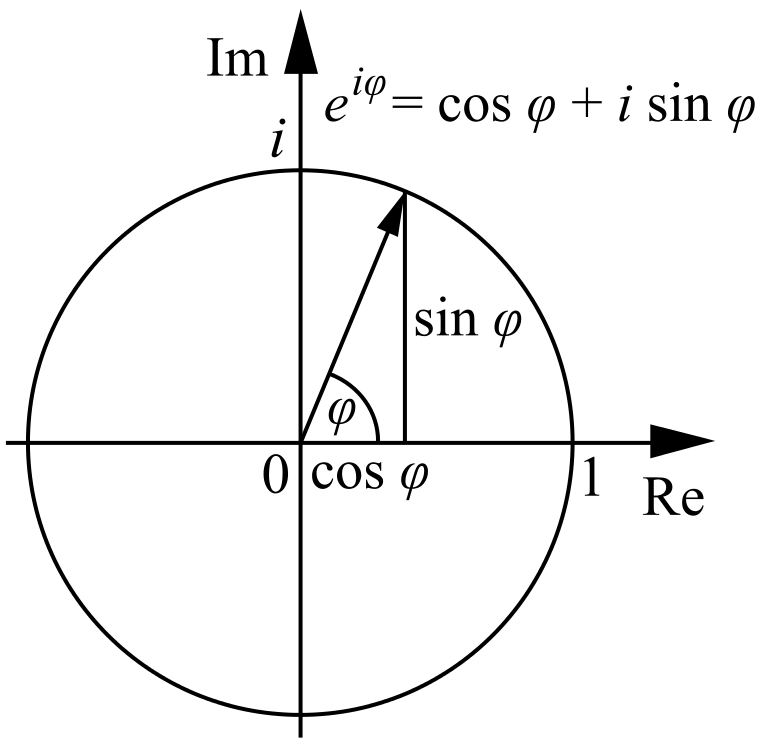
\includegraphics[width=0.85\linewidth]{example/Euler.png}
	\caption{This is a figure caption where you can describe the figure in words. It's always best to do this. No, really, you should strongly consider doing this. By Original: GuntherDerivative work: Wereon -- This file was derived from Euler's formula.png:, CC BY-SA 3.0, https://commons.wikimedia.org/w/index.php?curid=821342}
	\label{fig:fig_narrow}
\end{figure}

\begin{figure*}[ht]
	\centering
	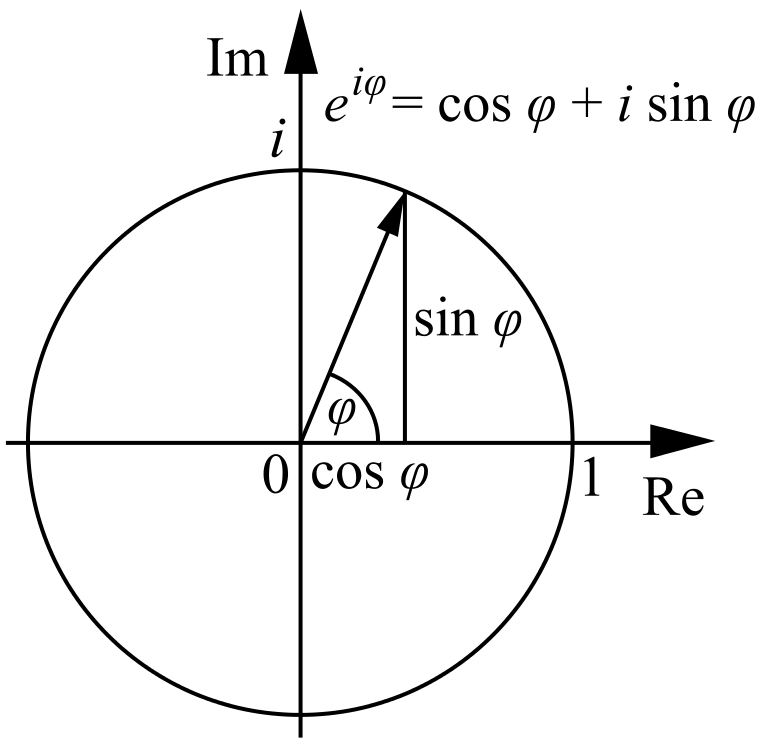
\includegraphics[width=0.45\linewidth]{example/Euler.png}
	\caption{This is a figure caption where you can describe the figure in words. It's always best to do this. No, really, you should strongly consider doing this. By Original: GuntherDerivative work: Wereon -- This file was derived from Euler's formula.png:, CC BY-SA 3.0, https://commons.wikimedia.org/w/index.php?curid=821342}
	\label{fig:fig_wide}
\end{figure*}

\subsection{Equations}
Equationing it up to demonstrate how to equation like a professional equationer,
\begin{equation}
	e^{i\pi} + 1 = \cos(\pi) + i\sin(\pi) + 1 = 0,
\end{equation}
and continuing on with more Kant. \kant. Time to demonstrate more section headings.

\subsection{Nonsense}

Thingy things that we always talk about.

\subsubsection{More Nonsense}

Because life isn't complete without more nonsense.

\subsubsection{Even More Nonsense}

Now it's just getting out of hand.

\section{Tables}

Life is difficult without tables, so we herein present a couple of example tables. They're nothing too exciting, but perhaps are essential for what you intend to write. 

\begin{table}[t]
	\centering
	\caption{Simple table for testing tabref.}
	\label{tab:table_narrow}
	\begin{tabular*}{0.85\linewidth}{l @{\extracolsep{\fill}} c l}
	\noalign{\smallskip}\hline\hline\noalign{\smallskip}
	Star & Data & Source \\
	\noalign{\smallskip}\hline\noalign{\smallskip}
	Star 1 &  0.5 & \citet{author1}  \\
	Star 2 &  0.4 & \citet{author2}  \\
	Star 3 &  0.3 & \citet{author3}  \\
	Star 4 &  0.2 & \citet{author4}  \\
	Star 5 &  0.1 & \citet{author5} \\
	\noalign{\smallskip}\hline
	\end{tabular*}
\end{table}

\begin{table*}[t]
	\centering
	\caption{Simple table for testing tabref.}
	\label{tab:table_wide}
	\begin{tabular*}{\linewidth}{l @{\extracolsep{\fill}} c l c l}
	\noalign{\smallskip}\hline\hline\noalign{\smallskip}
	Star & Data & Source & Extra Data & Source \\
	\noalign{\smallskip}\hline\noalign{\smallskip}
	Star 1 &  0.5 & \citet{author1} &  -1.0  & \citet{author1,author2,author5} \\
	Star 2 &  0.4 & \citet{author2} &  -2.0  & \citet{author2,author3}  \\
	Star 3 &  0.3 & \citet{author3} &  -3.0  & \citet{author2,author4}  \\
	Star 4 &  0.2 & \citet{author4} &  -4.0  & \citet{author4,author5}  \\
	Star 5 &  0.1 & \citet{author5} &  -5.0  & \citet{author3} \\
	\noalign{\smallskip}\hline
	\end{tabular*}
\end{table*}

\kant

\section*{Acknowledgments}
{Thank you to the world and myself. Mostly myself. Without me, I would have no results and no paper.}

\begin{thebibliography}{5}
\setlength{\itemsep}{0mm}
\small

\bibitem[\r{A}ngstrom et al.(1861)]{author1} \r{A}ngstrom, A., et al. 1861, Prestigous Journal, 1, 1

\bibitem[Celsius et al.(1906)]{author2} Celsius, A., et al. 1735, Great Book

\bibitem[Galilei(1630)]{author3} Galilei, G. 1630, Long-lost Book

\bibitem[Newton(1699)]{author4} Newton, I. 1899, Decent Book

\bibitem[Newton(1715)]{author5} Newton, I. \& Leibniz, G.~W. 1715, Yet-another Book

\end{thebibliography}

\end{document}
